\documentclass[12pt, a4paper, titlepage]{article}
\usepackage[a4paper,top=2.5cm,bottom=2cm,left=2cm,right=2cm]{geometry}
\usepackage[italian]{babel}
\usepackage[hidelinks]{hyperref}
\usepackage{graphicx}
\usepackage{algorithm}
\usepackage{capt-of}
\usepackage{amsmath}
\usepackage{longtable}
\usepackage{caption}
\usepackage{booktabs}
\usepackage{algpseudocode}
\usepackage{makecell}
\usepackage[utf8]{inputenc}
\usepackage{fixltx2e}
\usepackage{listings}
\usepackage{hyperref}
\usepackage{makecell}
\usepackage{changepage}
\usepackage{paracol}
\usepackage{siunitx}
\usepackage{lipsum}
\usepackage[swapnames]{frontespizio}
\usepackage{fancyhdr}
\usepackage{lastpage}
\usepackage{pdfpages}
\usepackage{tabularx}
\usepackage[acronym, nonumberlist]{glossaries}
\usepackage{amsmath}
\usepackage{tcolorbox}
\usepackage[newfloat]{minted}
\usepackage{animate}
\usepackage{lastpage}

\newenvironment{code}{\captionsetup{type=listing}}{}
\SetupFloatingEnvironment{listing}{name=Source Code}


\setcounter{secnumdepth}{3}
\makeglossaries	

\setlength{\parindent}{0mm}
\loadglsentries{glossaries}
\begin{document}

\newcommand{\HRule}{\rule{\linewidth}{0.5mm}} 
\pagenumbering{gobble}

\begin{center}
	
	\textsc{\LARGE Università degli Studi di Padova}\\[1cm] 
	
	
\includegraphics[height=5cm]{img/UniPd.png}\\[1cm]
	
	
\includegraphics[height=1.5cm, width = 9cm]{img/MathDip.png}\\
	\textsc{Dipartimento di Matematica ``Tullio Levi-Civita''}\\[1.2cm]
	\textsc{\Large Scuola di Scienze}\\[0.5cm] 
	
	\textsc{\large Corso di Laurea Magistrale in Informatica}\\[0.5cm] 
	
	\vspace{2.5cm}
	
	
	\HRule \\[0.4cm]
	{ \huge \bfseries Il Parallelismo in Terraform }\\[0.4cm]
	\HRule \\[1.5cm]
	
	
	\vspace{2.5cm}
	
	
	{\large 
		Francesco Antonio Migliorin \\ 
		1207422 \\
		Anno 2020/2021}\\[2cm]
	
	
	\vfill 
\end{center}
\tableofcontents
\newpage
\newpage
\listoffigures
\pagestyle{fancy}
\fancyhf{}
\rhead{Approfondimento}
\lhead{Linguaggi per il Global Computing}
\cfoot{\thepage}
\pagenumbering{arabic}
\clearpage

\section{Approfondimento Terraform}
Terraform\cite{terraform} è uno strumento di \gls{iac}, creato da \gls{hashicorp}, che fornisce una sintassi comune, chiamata \gls{hcl}, per interagire con più attori, che nella maggior parte dei casi sono cloud provider. É uno strumento molto giovane, infatti il 08/06/2021 é stata rilasciata la versione 1.0 di Terraform.

\begin{tcolorbox}
Questo approfondimento non vuole focalizzarsi sul linguaggio \gls{hcl} ma sul parallelismo di Terraform. Per questo motivo verranno trattate solamente le basi del linguaggio e del funzionamento di Terraform, necessarie per comprendere meglio l'argomento trattato. Non si prefigge quindi di essere una guida esaustiva.
\end{tcolorbox}

\subsection{Le basi di Terraform}
Terraform é uno strumento dichiarativo, scritto in \gls{go}, che utilizza il linguaggio di alto livello \gls{hcl} per descrivere l'infrastruttura cloud o on-premise. Terraform legge tutti i file, presenti in una directory, \texttt{.tf} che contengono la configurazione dell'infrastruttura e genera poi un piano, ovvero le azione necessarie per raggiungere lo "stato finale" desiderato, e successivamente  lo attua per eseguire l'effettivo provisioning dell'infrastruttura.

\subsubsection{I comandi principali}

\paragraph{Terraform Init}
Il comando \texttt{terraform init} viene utilizzato per inizializzare una directory contenente dei file di configurazione per terraform \texttt{.tf}.
Durante il processo di inizializzazione, i moduli e i \textit{providers} esterni vengono automaticamente rilevati cercando nel codice sorgente.  Vengono quindi referenziati i
moduli ed eventualmente scaricato il codice necessario per eseguirli, così come vengono inizializzati i provider, scaricando e installando il relativo plug-in, prima del loro primo utilizzo.

Durante l'inizializzazione vengono inoltre controllare le versioni dei moduli e dei provider per fare in modo che corrispondano.

\paragraph{Terraform Plan}
Il comando \texttt{terraform plan} viene utilizzato per creare un piano di esecuzione.
Terraform esegue il comando \texttt{refresh}, a meno che non sia disabilitato, e successivamente determina quali azioni sono necessarie per raggiungere lo "stato finale" specificato nei file di configurazione \texttt{.tf}.
Questo comando è un modo utile per poter verificare se il piano prodotto corrisponde alle modifiche che ci aspettavamo, senza apportare realmente, modifiche all'infrastruttura reale. Questo stato puó essere salvato in un file e passato al comando di \texttt{terraform apply}, in questo modo terraform eseguirà le operazioni nella stessa sequenza descritta nel piano.

\paragraph{Terraform Apply}
Il comando di \texttt{terraform apply} viene utilizzato per applicare le modifiche rilevate dal comando \texttt{plan} al fine di raggiungere lo stato descritto nella configurazione.
Durante l'esecuzione, a ogni task, Terraform scriverà lo stato attuale nel file \texttt{terraform.tfstate}. La funzione di questo file é quella di tenere memorizzata lo stato corrente della nostra infrastruttura, in questo modo Terraform sa cos'ha creato, cosa deve modificare e cosa deve distruggere.

\paragraph{Terraform Refresh}
Il comando \texttt{terraform refresh} viene utilizzato per riconciliare l'infrastruttura reale con lo stato di cui Terraform è a conoscenza (lo stato per Terraform si trova nel file \texttt{terraform.tfstate}).
In questo modo terraform mappa le modifiche che sono state fatte all'infrastruttura e aggiorna il file \texttt{terraform.tfstate}.

\paragraph{Terraform Destroy}
Il comando \texttt{terraform destroy} viene utilizzato per distruggere l'infrastruttura descritta nel file \texttt{terraform.tfstate}. Il suo comportamento é analogo al comando \texttt{terraform apply}, tuttavia al posto di creare risorse le distrugge.

\paragraph{Terraform Import}
Terraform è in grado di importare componenti di infrastruttura giá esistenti. Questo permette di portare elementi esistenti sotto la gestione di Terraform, che verranno mappati con la configurazione desiderata e inseriti nel file \texttt{terraform.tfstate}.

\subsubsection{I principi del linguaggio}

\paragraph{Providers}
La risorsa principale messa a disposizione da terraform sono i \textit{providers}. Questi si occupano dell'interazione tra Terraform e il suo target, che normalmente avviene tramite API.

\begin{figure}[ht!]
	\centering
	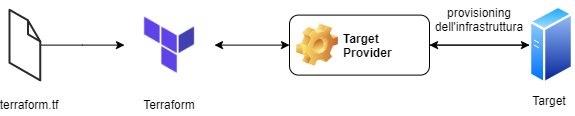
\includegraphics[width=120mm]{./img/provider.png}
	\caption{Architettura dei provider}
	\label{fig:provider-architecture}
\end{figure}

I \textit{providers} sono distribuiti separatamente da Terraform stesso e sono anch'essi scritti in \gls{go}. Tutti quelli disponibili, possono essere trovati nel loro registro ufficiale\cite{terraform_registry}. Ciascun provider aggiunge risorse e/o dati che Terraform può gestire. Senza \textit{providers}, Terraform non può gestire nessun tipo di infrastruttura.

 \begin{code}
	\begin{minted}[mathescape, linenos]{terraform}
provider "aws" {
  region     = "us-west-2"
  access_key = "my-access-key"
  secret_key = "my-secret-key"
}
	\end{minted}
	\captionof{listing}{Esempio di dichiarazione di un provider}
\end{code}

\paragraph{Resources}
Ogni blocco di risorsa dichiara che si desidera che un particolare oggetto dell'infrastruttura esista con le impostazioni fornite in input.

 \begin{code}
	\begin{minted}[mathescape, linenos]{terraform}
resource "aws_instance" "vm" {
  ami           = "ami-a1b2c3d4"
  instance_type = "t2.micro"
}
	\end{minted}
	\captionof{listing}{Esempio di dichiarazione di una risorsa}
\end{code}
\bigskip

Quando Terraform crea un nuovo oggetto dell'infrastruttura, rappresentato da un blocco risorsa, l'identificatore per quell'oggetto reale viene salvato nel file \texttt{terraform.tfstate}. Questo consentirà l'aggiornamento e la distruzione della risorsa o eventuali modifiche future. Se il blocco risorsa é già associato ad un elemento dello stato, Terraform confronta la configurazione effettiva dell'oggetto, con i parametri forniti dalla configurazione e se necessario, aggiorna l'oggetto in modo che corrisponda alla configurazione.

É possibili inoltre, utilizzare le informazioni di una risorsa per configurare altre risorse. Utilizzando la sintassi \texttt{<RESOURCE TYPE>.<NAME>.<ATTRIBUTE>} andiamo a fare riferimento a un attributo di una determinata risorsa. In questo modo possiamo andare a recuperare le informazioni che non possono essere conosciute fino a quando la risorsa non viene effettivamente creata, andando quindi a creare una dipendenza implicita tra due risorse. Terraform analizza qualsiasi espressione all'interno di un blocco risorsa, per trovare riferimenti ad altre risorse e trasforma questi riferimenti in requisiti di ordinamento impliciti durante la creazione, l'aggiornamento o la distruzione delle risorse. 

 \begin{code}
	\begin{minted}[mathescape, linenos]{terraform}
resource "tls_private_key" "global_key" {
  algorithm = "RSA"
  rsa_bits  = 2048
}
	
resource "aws_key_pair" "test" {
  key_name   = "test-key"
  public_key      = tls_private_key.global_key.public_key_openssh
}
	\end{minted}
	\captionof{listing}{In questo esempio vediamo come la risorsa \texttt{aws\_key\_pair.test} dipenda dal risultato di \texttt{tls\_private\_key.global\_key}}
\end{code}
\bigskip
La maggior parte delle risorse di una configurazione non ha alcuna dipendenza particolare oppure é sempre implicita e Terraform puó lavorare in modo parallelo. Tuttavia, alcune dipendenze non possono essere riconosciute, da Terraform, implicitamente nella configurazione. In questi casi, possiamo creare una dipendenza esplicata utilizzando il meta-argomento \texttt{depend\_on}.

 \begin{code}
	\begin{minted}[mathescape, linenos]{terraform}
resource "aws_s3_bucket" "bucket" {
  acl    = "private"
}

resource "aws_instance" "vm" {
  ami           = "ami-a1b2c3d4"
  instance_type = "t2.micro"

  depends_on = [aws_s3_bucket.bucket]
}
	\end{minted}
	\captionof{listing}{In questo esempio vediamo come la risorsa \texttt{aws\_instance.vm} dipenda, in modo esplicito, dal risultato di \texttt{aws\_s3\_bucket.bucket}}
\end{code}

\paragraph{Data Sources} Un blocco di dati richiede che Terraform legga da una determinata sorgente dati. In questo modo possiamo leggere informazioni dall'esterno e importarle per utilizzarle in Terraform.

 \begin{code}
	\begin{minted}[mathescape, linenos]{terraform}
data "aws_ami" "example" {
  most_recent = true

  owners = ["self"]
}
	\end{minted}
	\captionof{listing}{Esempio di dichiarazione di un data sources}
\end{code}
\bigskip

\begin{tcolorbox}
I \textit{Data Sources} hanno lo stesso comportamento e vengono trattati da Terraform come se fossero delle \textit{Resources}. L'unica differenza é che i blocchi di dati vengono effettivamente eseguiti durante il comando \texttt{terraform plan} per rilevare eventuali difformità. Per questo motivo d'ora in avanti verranno considerati come se fossero delle \textit{Resources}, se non diversamente menzionato.
\end{tcolorbox}

\paragraph{Provisioners} I \textit{provisioners} possono essere utilizzati per effettuare azioni specifiche sulla macchina locale o su una remota e posso essere creati solamente all'interno di un blocco risorse.

 \begin{code}
	\begin{minted}[mathescape, linenos]{terraform}
resource "aws_instance" "vm" {
  ami           = "ami-a1b2c3d4"
  instance_type = "t2.micro"

  provisioner "local-exec" {
    command = "echo The server's IP address is ${self.private_ip}."
  }
}
	\end{minted}
	\captionof{listing}{Esempio di dichiarazione di un provisioner}
\end{code}
\bigskip

Per impostazione predefinita, i \textit{provisioners} vengono eseguiti quando viene creata la risorsa in cui sono definiti e solamente durante l'esecuzione del comando \texttt{terraform apply}.
\bigskip

Se un provisioner fallisce, la risorsa a cui é associato viene contrassegnata come "contaminata". Una risorsa contaminata sarà pianificata per la distruzione e successivamente verrá riscreata al prossimo comando \texttt{terraform apply}. Terraform esegue questa procedura perché ritiene di aver lasciato la risorsa contaminata in uno stato "parzialmente configurata" e quindi l'unico modo per garantire la corretta creazione di una risorsa contaminata è la sua ricreazione. É possibile però disabilitare questo comportamento tramite il meta-argomento \texttt{on\_failure}.
\bigskip

É possibile dire a un \textit{provisioner} di essere eseguito durante la fase di distruzione, invece che di creazione, mediante il meta-argomento \texttt{when = destroy}. Durante la fase di distruzione i \textit{provisioner} vengono eseguiti prima che la risorsa venga distrutta. Se falliscono, Terraform si bloccherà  con un errore.

 \begin{code}
	\begin{minted}[mathescape, linenos]{terraform}
resource "aws_instance" "vm" {
  ami           = "ami-a1b2c3d4"
  instance_type = "t2.micro"

  provisioner "local-exec" {
    when       = destroy
    command = "echo The server's ${self.private_ip} will be destroyed."
  }
}
	\end{minted}
	\captionof{listing}{Esempio di dichiarazione di un provisioner che verrà eseguito in fase di distruzione}
\end{code}
\bigskip

È possibile specificare più \textit{provisioners} all'interno di una risorsa, quest'ultimi verranno eseguiti nell'ordine in cui sono definiti nel file di configurazione. É possibile combinare i \textit{provisioners} di creazione e distruzione nella stessa risorsa, si occuperà Terraform di eseguire solo quelli validi il comando in esecuzione.

\begin{code}
	\begin{minted}[mathescape, linenos]{terraform}
resource "aws_instance" "vm" {
  ami           = "ami-a1b2c3d4"
  instance_type = "t2.micro"

  provisioner "local-exec" {
    command = "echo first"
  }

  provisioner "local-exec" {
    command = "echo second"
  }
}
	\end{minted}
	\captionof{listing}{Esempio di dichiarazione di un multi-provisioner}
\end{code}
\bigskip

\begin{tcolorbox}
Terraform sconsiglia l'utilizzo dei \textit{provisioners} e consiglia di utilizzarli come ultima risorsa, quando non si hanno altre alternative. 
\end{tcolorbox}

\paragraph{Modules} 
I moduli sono dei contenitori di risorse, ovvero consistono in una raccolta di file \texttt{.tf} presenti in una directory.

I moduli sono l'unico modo per creare pacchetti di codice riutilizzabile, mettendo insieme le configurazioni delle risorse con Terraform. Esiste sempre almeno un modulo, noto come \textit{root module}, che consiste nelle risorse definite nei file \texttt{.tf} nella directory dove viene eseguito Terraform.

Un modulo Terraform può chiamare altri moduli per includere le loro risorse nella configurazione,  questi sono chiamati \textit{child modules} e possono essere chiamati più volte all'interno della stessa configurazione o con configurazioni diverse. 

\begin{code}
	\begin{minted}[mathescape, linenos]{terraform}
module "eks" {
  source  = "terraform-aws-modules/eks/aws"
  version = "17.1.0"
  # insert the 9 required variables here
}
	\end{minted}
	\captionof{listing}{Esempio di dichiarazione del \textit{child modules} \texttt{terraform-aws-eks} v17.1.0 \cite{terraform_eks}}
\end{code}
\bigskip

Durante l'esecuzione di un modulo, Terraform lo tratta come una scatola nera, quindi conoscendo gli input sappiamo quali output aspettarci ma il come quell'input viene trasformato in quell'output, non é dato sapersi. Lo stesso vale per le risorse all'interno del modulo che non hanno alcuna conoscenza dell'ambiente esterno. Per questo motivo é molto importante progettare bene gli input e gli output durante la creazione di un modulo.

\begin{code}
	\begin{minted}[mathescape, linenos]{terraform}
variable "name" {
  description = "The name of the virtual machine created"
  type          = string
  default      = "pippo"
}
	\end{minted}
	\captionof{listing}{Esempio di dichiarazione di un input per un modulo}
\end{code}
\bigskip

\begin{code}
	\begin{minted}[mathescape, linenos]{terraform}
output "private_ip" {
  description = "The created virtual machines private ip"
  value         = aws_instance.vm.private_ip
}
	\end{minted}
	\captionof{listing}{Esempio di dichiarazione di un output per un modulo}
\end{code}
\bigskip

I moduli possono essere caricati dal filesystem locale oppure Terraform può scaricare i moduli dal registro ufficiale\cite{terraform_registry} o da uno privato. Ciò rende possibile pubblicare i propri moduli che altri potranno utilizzare o utilizzare i moduli che altri hanno pubblicato.

\subsection{Il parallelismo in Terraform}
I grafici sono strutture matematiche utilizzate per modellare le relazioni presenti  tra gli oggetti. Possiamo quindi pensare alle moderne infrastrutture come grafici: le risorse computazionali normalmente dipendono dalle risorse di rete, che a loro volta dipendono dalle risorse di sicurezza, etc... 
Sfruttando questa teoria Terraform crea un grafico per modellare le relazioni tra le risorse, in modo che i provider possano gestire e modificare in sicurezza le risorse dell'infrastruttura, prevedendo, in questo modo, i cambiamenti con conseguenze impreviste.
Un altro vantaggio implicito nell'utilizzare Terraform é la possibilità di avere una mappa di tutte le relazioni dell'infrastruttura, cosa impossibile su larga scala. Utilizzando questa filosofia Terraform é in grado di eseguire in modo parallelo piú operazioni senza incorrete in rischi.

\subsubsection{I tipi di nodo}
Ci sono solo tre tipi di nodi che possono esistere all'interno del grafico creato da Terraform:

\begin{itemize}
	\item \textit{Nodo risorsa:} rappresenta una singola \textit{resource};

	\item \textit{Nodo di configurazione del provider:}  rappresenta il tempo necessario 			per configurare completamente un \textit{provider}. Questo viene creato quando é presente un blocco di configurazione del provider;

	\item \textit{Meta-nodo risorsa:} rappresenta un gruppo di risorse, ma non 				rappresenta alcuna azione da solo. Questo viene fatto per comodità sulle dipendenze e 	per creare un grafico più semplice. Questo nodo è presente solo per le risorse che 			hanno un parametro \texttt{count}/\texttt{for\_each} maggiore di 1.
\end{itemize}
 
\subsubsection{Costruzione del grafo} 
La costruzione del grafico avviene in una serie di passaggi sequenziali:

\begin{enumerate}
	\item I \textit{nodi risorsa} vengono aggiunti in base alla configurazione rilevata automaticamente. Se è presente una difformità rispetto al piano o allo stato fornito, vengono aggiunti dei metadati a ciascun \textit{nodo risorsa}, in modo da tener traccia del cambiamento;

	\item Le risorse vengono mappate ai \textit{provisioners}, se questi sono stati definiti. Questa operazione viene eseguita dopo la creazione di tutti i \textit{nodi risorsa}, in modo che le risorse con lo stesso tipo di \textit{provisioner} possano condividere la stessa implementazione;
	
	\item Vengono create le dipendenze esplicite, quindi quelle con esplicitato il parametro \texttt{depend\_on};

	\item Se è presente uno stato, tutte le risorse "orfane" vengono aggiunte al grafico. Per "risorse orfane" si intende tutte le risorse che non sono più presenti nella 	configurazione ma presenti nel file di stato \texttt{terraform.tfstate}. Alle "risorse  orfane" non è associata alcun \textit{provider}, poiché la configurazione di quest'ultimo non viene memorizzata nel file di stato \texttt{terraform.tfstate};

	\item Le risorse vengono mappate ai \textit{provider} definiti nella configurazione. I \textit{nodi di configurazione del provider} vengono creati per i \textit{provider} e vengono creati degli archi in modo tale che le risorse dipendano dalla configurazione del rispettivo \textit{provider};

	\item Terraform, al fine di creare le dipendenze implicite, analizza l'attuale 	configurazione di risorse e provider per individuarne le dipendenze. Per fare ció trasforma gli attributi della risorsa in dipendenze, creando un arco con la risorsa a cui fa riferimento; 

	\item Viene creato il nodo radice, detto \textit{root}. Il nodo radice punta a tutte le risorse e viene creato in modo che ci sia unico. Durante l'attraversamento del grafico il nodo radice viene ignorato. Insieme al nodo radice vengono creati anche una serie di nodi per le operazioni interne di Terraform, tutti questi nodi iniziano con il prefisso \texttt{[root]};

	\item Terraform attraversa tutti i \textit{nodi risorsa} e gli analizza per trovare quelli che devono essere distrutti. Questi \textit{nodi risorsa} vengono divisi in due: un nodo che distruggerà la risorsa e un altro che creerà la risorsa (se questa deve essere ricreata). Questo viene fatto perché l'ordine di distruzione è spesso diverso dall'ordine di creazione e quindi non possono essere rappresentati da un singolo nodo del grafico;

	\item Il grafico viene convalidato per verificare che non ci siano cicli e che contenga un unico nodo radice. 
\end{enumerate}

\subsubsection{Controllo dei cicli}

Per controllare la presenza di cicli Terraform utilizza l'Algoritmo di Tarjan, come possiamo vedere dal suo codice sorgente \cite{terraform_tarjan}, liberamente accessibile su Github.

\begin{figure}[ht!]
	\centering
	\animategraphics[width=\textwidth]{12}{./img/tarjan_algorithm_animation/frame-}{0}{16}
	\caption{Animazione dell'applicazione dell'algoritmo di Tarjan su un grafo}
	\textbf{Fonte:} \url{https://wikipedia.org/wiki/File:Tarjan%27s_Algorithm_Animation.gif}
	\label{fig:cycle}
\end{figure}

L'algoritmo di Tarjan , prende il nome del suo inventore Robert Tarjan e l'idea si basa sul fatto che la ricerca \gls{dfs} produce in output un albero/foresta. Si potrà quindi andare a trovare le componenti \gls{ssc}, come sotto-alberi dell'albero/foresta di partenza. Qualsiasi vertice che non fa parte di un ciclo forma, da solo, una \gls{ssc}: per esempio, un qualsiasi vertice di un grafo aciclico. Per fare ció, a ogni nodo è assegnato un indice, in base alla profondità della ricerca. Durante la ricerca \gls{dfs} viene calcolato anche il valore \textit{lowlink}, ovvero l'indice che deve avere per essere raggiungibile dalla radice. Quindi un vertice é la radice di una \gls{ssc} se e solo se il suo indice corrisponde al \textit{lowlink} degli altri nodi. Nel caso peggiore la complessità é pari a $O(|E| + |V|)$.

\subsubsection{Attraversamento del grafo} 
Per percorrere il grafico, viene eseguito un attraversamento con un algoritmo \gls{dfs} eseguito in parallelo. In questo modo un nodo puó essere percorso non appena vengono percorse tutte le sue dipendenze.

La quantità di parallelismo è limitata a un valore massimo, impostato utilizzando il flag \texttt{-parallelism} da linea di comando, per evitare che troppe operazioni simultanee sovraccaricano le risorse della macchina che esegue Terraform.

\begin{tcolorbox}
É bene precisare che l'attraversamento del grafo avviene in modo parallelo e non concorrente, come precisa anche il suo creatore Mitchell Hashimoto \cite{github_issue_11766}.
\end{tcolorbox}

\subsubsection{Il comando \texttt{graph}}

Il comando \texttt{terraform graph} viene utilizzato per generare una rappresentazione visiva, in formato \gls{dot}, della configurazione attuale.

Il flag \texttt{-type} può essere usato per controllare il tipo di grafico mostrato. Terraform crea grafici in base al tipo di operazione: \texttt{plan}, \texttt{destroy}, \texttt{apply}, \texttt{validate}, \texttt{import}, \texttt{refresh}.  Un argomento molto utile é \texttt{-draw-cycles}  che va ad evidenziare tutti i cicli presenti nel grafico.

\subsubsection{Esempio di grafo} 
Vediamo insieme un esempio di output del comando \texttt{terraform graph}. Per questo esempio é stata utilizzata la versione 1.0.3 della terraform cli, disponibile qui \cite{terraform_cli}, e la versione 3.52.0 del provider terraform \gls{aws}, disponibile qui \cite{terraform_aws}.

Prendiamo il seguente codice come esempio, andando a creare un file \texttt{demo.tf}:
\begin{code}
	\begin{minted}[mathescape, linenos]{terraform}
terraform {
  required_providers {
    aws = {
      source  = "hashicorp/aws"
      version = "3.52.0"
    }
  }
}

provider "aws" {
  region = "us-west-2a"
}

data "aws_ami" "ubuntu" {
  most_recent = true

  filter {
    name   = "name"
    values = ["ubuntu/images/hvm-ssd/ubuntu-focal-20.04-amd64-server-*"]
  }

  filter {
    name   = "virtualization-type"
    values = ["hvm"]
  }

  owners = ["099720109477"]
}

resource "aws_instance" "vm" {
  ami               = data.aws_ami.ubuntu.id
  availability_zone = "us-west-2a"
  instance_type     = "t2.micro"
}

resource "aws_ebs_volume" "disk" {
  availability_zone = "us-west-2a"
  size              = 1
}

resource "aws_volume_attachment" "ebs_att" {
  device_name = "/dev/sdh"
  volume_id   = aws_ebs_volume.disk.id
  instance_id = aws_instance.vm.id
}
	\end{minted}
	\captionof{listing}{Esempio di codice terraform}
\end{code}
\bigskip

Di seguito la spiegazione passo passo del codice sopra mostrato:

\begin{code}
	\begin{minted}[mathescape, linenos]{terraform}
terraform {
  required_providers {
    aws = {
      source  = "hashicorp/aws"
      version = "3.52.0"
    }
  }
}
	\end{minted}
	\captionof{listing}{Blocco di codice \texttt{required\_providers} \label{code:providers}}
\end{code}
\bigskip

In questo esempio con il blocco di codice \ref{code:providers} andiamo a fornire a Terraform una lista di \textit{providers}, andando a specificare da quale registro reperire il codice sorgente e l'eventuale versione  che vogliamo utilizzare. Questo blocco di codice é opzionale e se non valorizzato terraform troverà in automatico i \textit{providers}, andando a prendere sempre la versione \textit{lastest} dal registro ufficiale\cite{terraform_registry}. 

\begin{code}
	\begin{minted}[mathescape, linenos]{terraform}
provider "aws" {
  region = "us-west-2a"
}
	\end{minted}
	\captionof{listing}{Blocco di codice \texttt{provider}}
	\label{code:provider}
\end{code}
\bigskip

Nel blocco di codice \ref{code:provider} andiamo a inizializzare il provider \gls{aws}, in questo esempio andiamo a definire solo il parametro obbligatorio \texttt{region}. Se si desidera provare ad effettuare un \texttt{terraform apply} é necessario autenticarsi tramite variabili d'ambiente come descritto qui \cite{terraform_aws_auth}.

\begin{code}
	\begin{minted}[mathescape, linenos]{terraform}
data "aws_ami" "ubuntu" {
  most_recent = true

  filter {
    name   = "name"
    values = ["ubuntu/images/hvm-ssd/ubuntu-focal-20.04-amd64-server-*"]
  }

  filter {
    name   = "virtualization-type"
    values = ["hvm"]
  }

  owners = ["099720109477"]
}
	\end{minted}
	\captionof{listing}{Blocco di codice \texttt{aws\_ami.ubuntu}}
	\label{code:ami}
\end{code}
\bigskip

Tramite il blocco di codice \ref{code:ami} indichiamo a Terraform di reperire delle informazioni da \gls{aws}, riguardanti una precisa versione di ubuntu. Questi dati ci serviranno poi per avere il corretto \gls{ami} da passare alla virtual machine che creeremo.

\begin{code}
	\begin{minted}[mathescape, linenos]{terraform}
resource "aws_instance" "vm" {
  ami               = data.aws_ami.ubuntu.id
  availability_zone = "us-west-2a"
  instance_type     = "t2.micro"
}
	\end{minted}
	\captionof{listing}{Blocco di codice \texttt{aws\_instance.vm}}
	\label{code:instance}
\end{code}
\bigskip

Tramite il blocco di codice \ref{code:instance} diciamo a Terraform che vogliamo una virtual machine di tipo \textit{t2.micro}\cite{aws_t_2} nella zona \textit{us-west-2a}. Per il sistema operativo utilizziamo l'\gls{ami} ottenuto dal blocco di codice precedente, andando in questo modo a creare una dipendenza implicita tra le due risorse.

\begin{code}
	\begin{minted}[mathescape, linenos]{terraform}
resource "aws_ebs_volume" "disk" {
  availability_zone = "us-west-2a"
  size              = 1
}
	\end{minted}
	\captionof{listing}{Blocco di codice \texttt{aws\_ebs\_volume.disk}}
	\label{code:volume}
\end{code}
\bigskip

Tramite il blocco di codice \ref{code:volume} diciamo a Terraform che vogliamo un disco di 1GB nella zona \textit{us-west-2a}.

\begin{code}
	\begin{minted}[mathescape, linenos]{terraform}
resource "aws_volume_attachment" "ebs_att" {
  device_name = "/dev/sdh"
  volume_id   = aws_ebs_volume.disk.id
  instance_id = aws_instance.vm.id
}
	\end{minted}
	\captionof{listing}{Blocco di codice \texttt{aws\_volume\_attachment.ebs\_att}}
	\label{code:attachment}
\end{code}
\bigskip

Tramite il blocco di codice \ref{code:attachment} diciamo a Terraform che vogliamo attaccare il disco creato alla macchina virtuale che abbiamo creato.
\bigskip

Nella stessa directory dove abbiamo creato il file \texttt{demo.tf} andiamo a lanciare il comando \texttt{terraform init} per inizializzare la cartella e scaricare il codice necessario per eseguire il provider \gls{aws}. Una volta che il comando \texttt{terraform init} é terminato, possiamo andare a vedere il grafico che Terraform genera, utilizzando il comando \texttt{terraform graph}.

\begin{code}
	\begin{minted}[mathescape, linenos,fontsize=\tiny]{dot}
digraph {
        compound = "true"
        newrank = "true"
        subgraph "root" {
                "[root] aws_ebs_volume.disk (expand)" [label = "aws_ebs_volume.disk", shape = "box"]
                "[root] aws_instance.vm (expand)" [label = "aws_instance.vm", shape = "box"]
                "[root] aws_volume_attachment.ebs_att (expand)" [label = "aws_volume_attachment.ebs_att", shape = "box"]
                "[root] data.aws_ami.ubuntu (expand)" [label = "data.aws_ami.ubuntu", shape = "box"]
                "[root] provider[\"registry.terraform.io/hashicorp/aws\"]" [label = "provider[\"registry.terraform.io/hashicorp/aws\"]", shape = "diamond"]
                "[root] aws_ebs_volume.disk (expand)" -> "[root] provider[\"registry.terraform.io/hashicorp/aws\"]"
                "[root] aws_instance.vm (expand)" -> "[root] data.aws_ami.ubuntu (expand)"
                "[root] aws_volume_attachment.ebs_att (expand)" -> "[root] aws_ebs_volume.disk (expand)"
                "[root] aws_volume_attachment.ebs_att (expand)" -> "[root] aws_instance.vm (expand)"
                "[root] data.aws_ami.ubuntu (expand)" -> "[root] provider[\"registry.terraform.io/hashicorp/aws\"]"
                "[root] meta.count-boundary (EachMode fixup)" -> "[root] aws_volume_attachment.ebs_att (expand)"
                "[root] provider[\"registry.terraform.io/hashicorp/aws\"] (close)" -> "[root] aws_volume_attachment.ebs_att (expand)"
                "[root] root" -> "[root] meta.count-boundary (EachMode fixup)"
                "[root] root" -> "[root] provider[\"registry.terraform.io/hashicorp/aws\"] (close)"
        }
}
	\end{minted}
	\captionof{listing}{Risultato del comando \texttt{terraform graph}}
\end{code}
\bigskip

Di per se questo output non é molto significativo, infatti vediamo come con solamente sei blocchi di codice abbiamo un output di venti righe davvero poco leggibili. Fortunatamente é possibile convertire questo output, che ricordiamo essere nel formato standard \gls{dot}, in un output grafico. Per farlo possiamo usare uno dei tanti tool da linea di comando oppure online. Per questo approfondimento ho utilizzato il tool da linea di comando di Graphviz \cite{graphviz}.

\begin{figure}[ht!]
	\centering
	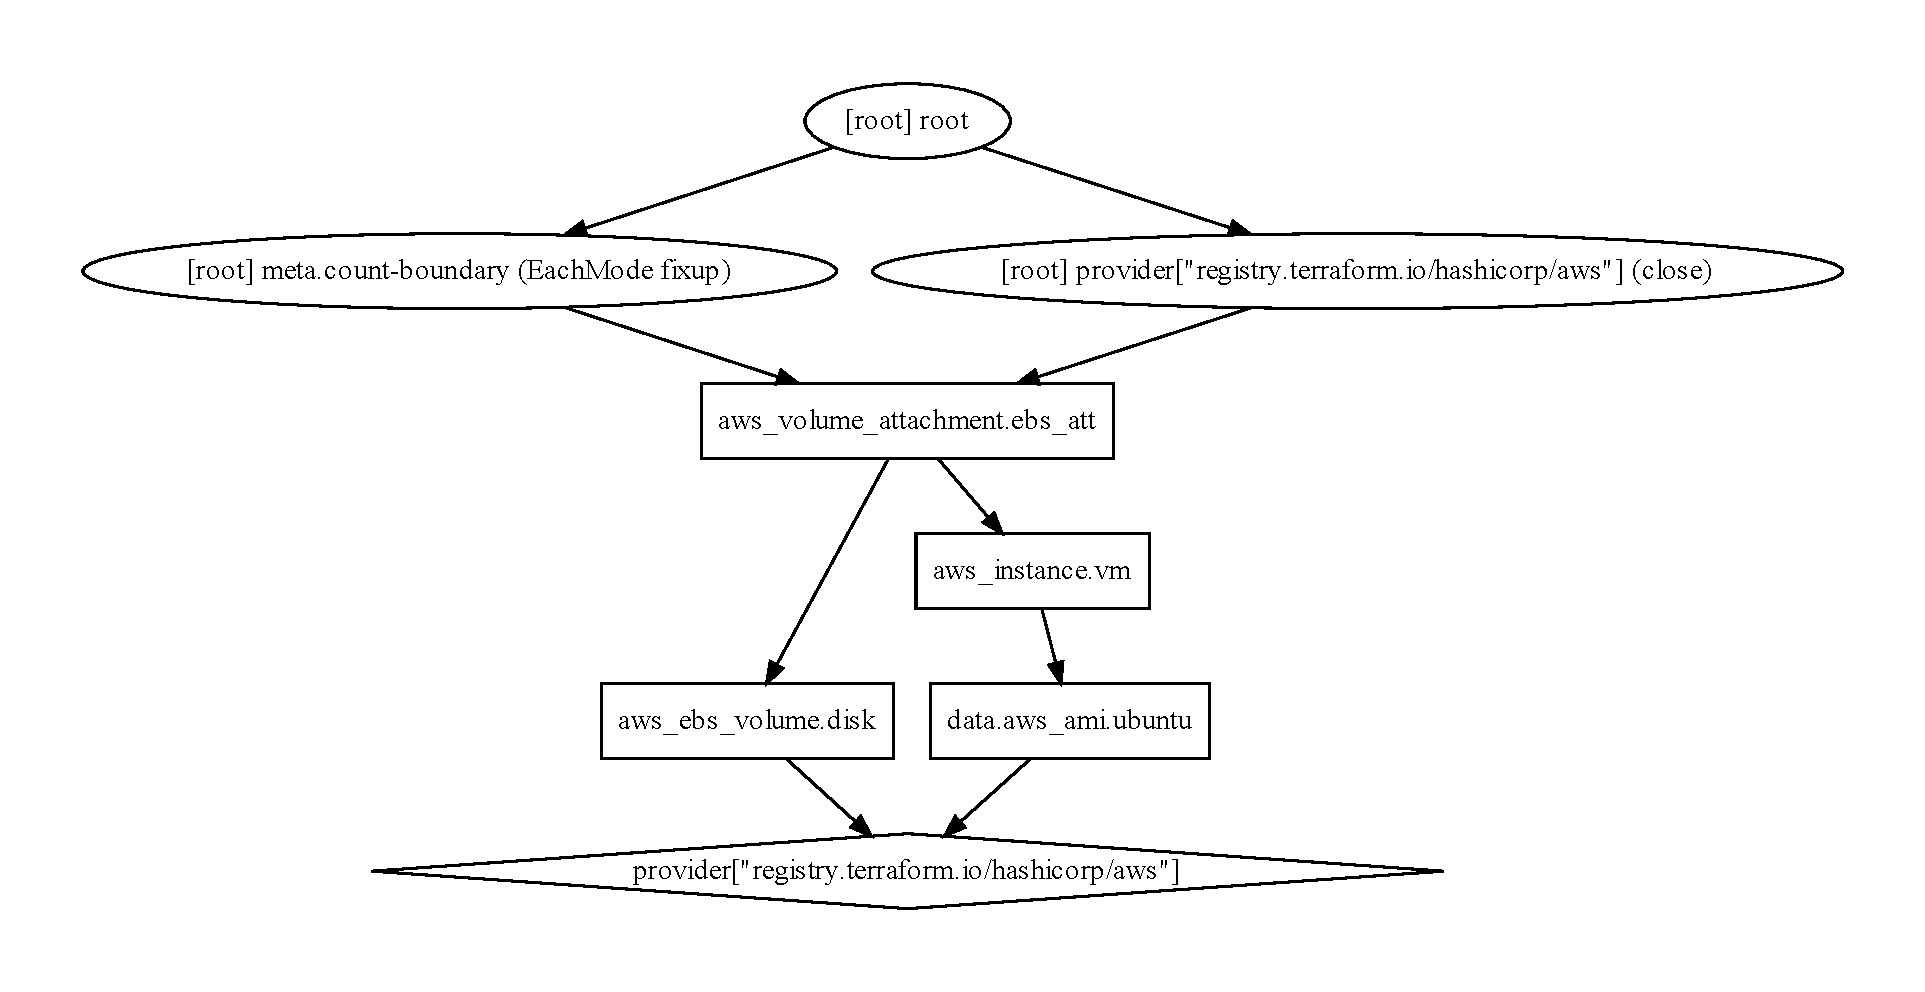
\includegraphics[width=160mm]{./img/graph.pdf}
	\caption{Visualizzazione grafica del risultato del comando \texttt{terraform graph}}
	\label{fig:graph}
\end{figure}

Dal grafico notiamo subito due nodi con il prefisso \texttt{[root]} collegati al \textit{nodo di root}. Questi sono dei nodi che ha aggiunto Terraform, infatti sono operazioni interne di terraform che questo andrà a fare e che in futuro verranno nascoste o avranno un output apposito per essere mostrare \cite{github_issue_14511}.

Simulando il comportamento di Terraform partiamo dal nodo

\texttt{[root] provider["registry.terraform.io/hashicorp/aws"]} dove avviene l'inizializzazione del provider. Successivamente in modo parallelo vengono eseguiti i nodi \texttt{aws\_ebs\_volume.disk} e \texttt{data.aws\_ami.ubuntu}, al termine di quest'ultimo viene risolta la dipendenza per il nodo \texttt{aws\_instance.vm} e viene quindi eseguito.
Risolte tutte le dipendenze precedenti viene eseguito l'ultimo nodo \texttt{aws\_volume\_attachment.ebs\_att}. 

\clearpage
\subsection{Conclusione}

\paragraph{Aspetti Positivi}
\begin{itemize}
	\item Crea o modifica l'infrastruttura in modo rapido e affidabile;
	\item Favorisce il riutilizzo del codice tramite l'utilizzo di moduli;
	\item Possiede un'ottima community che da supporto e pubblica molte soluzione sul registro ufficiale \cite{terraform_registry}; 
	\item Da la possibilità di vedere in anteprima i cambiamenti, grazie al comando \texttt{terraform plan}.
\end{itemize}
 
\paragraph{Aspetti Negativi}
\begin{itemize}
	\item Nessuna funzionalità di rollback, per realizzarlo é necessario tornare alla versione precedente del codice;
	\item ll linguaggio \gls{hcl} é semplice ma molto limitato, spesso per semplici azioni é necessario scrivere diverse linee di codice;
	\item L'output degli errori é spesso criptico o impreciso.
\end{itemize}

In sostanza Terraform é ancora un linguaggio molto giovane e poco flessibile, tuttavia non ci sono altre alternative in grado di garantire lo stesso livello di servizio ed affidabilità.

\nocite{*}
\newpage
\pagenumbering{gobble}
\printglossaries
\newpage
\bibliography{./bibliographic.bib} 
\bibliographystyle{ieeetr}

\end{document}